\renewcommand{\mapa}{Poglavja/Slike/informacija ranga}

\begin{figure}[!ht]
    \begin{subfigure}{0.325\linewidth}
        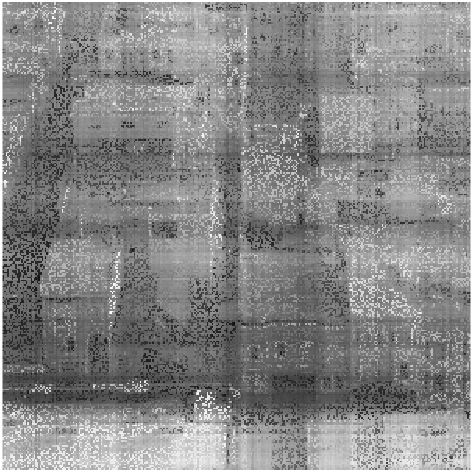
\includegraphics[width=\linewidth]{\mapa/rezLMaFit1.png}
        \caption{Rekonstrukcija s parametrom 1.}
    \end{subfigure}
    \hfill
    \begin{subfigure}{0.325\linewidth}
        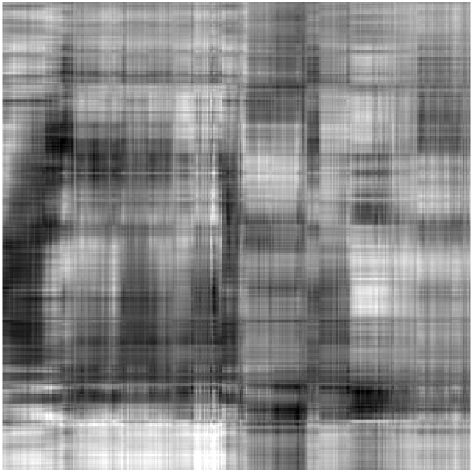
\includegraphics[width=\linewidth]{\mapa/rezLMaFit5.png}
        \caption{Rekonstrukcija s parametrom 5.}
    \end{subfigure}
    \hfill
    \begin{subfigure}{0.325\linewidth}
        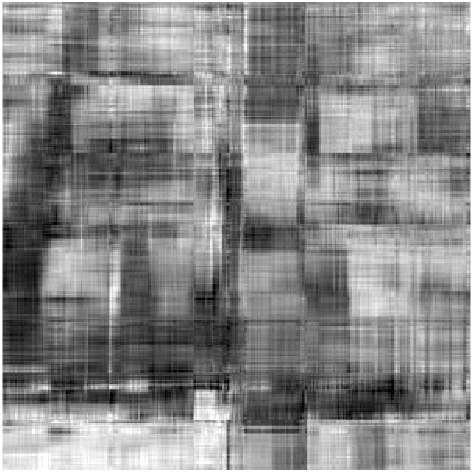
\includegraphics[width=\linewidth]{\mapa/rezLMaFit10.png}
        \caption{Rekonstrukcija s parametrom 10.}
    \end{subfigure}

    \begin{subfigure}{0.325\linewidth}
        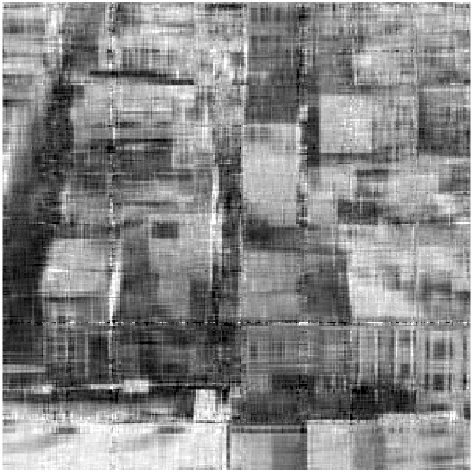
\includegraphics[width=\linewidth]{\mapa/rezLMaFit22.png}
        \caption{Rekonstrukcija s parametrom 22.}
    \end{subfigure}
    \hfill
    \begin{subfigure}{0.325\linewidth}
        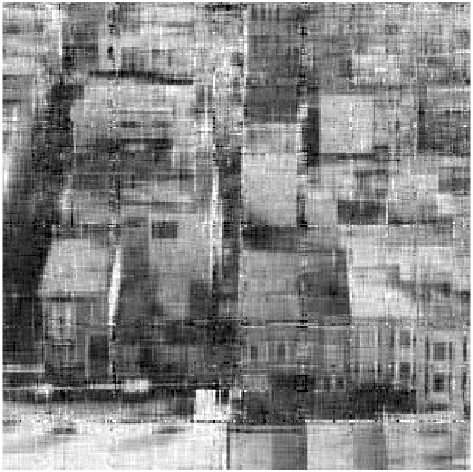
\includegraphics[width=\linewidth]{\mapa/rezLMaFit25.png}
        \caption{Rekonstrukcija s parametrom 25.}
    \end{subfigure}
    \hfill
    \begin{subfigure}{0.325\linewidth}
        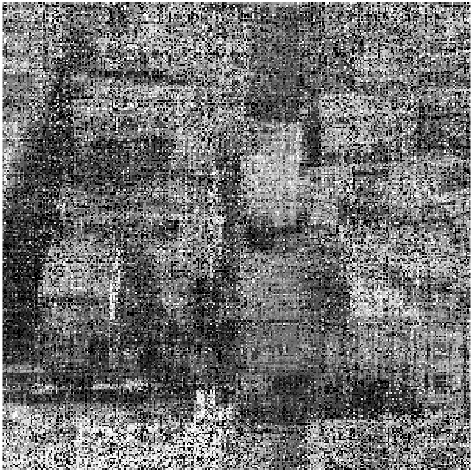
\includegraphics[width=\linewidth]{\mapa/rezLMaFit60.png}
        \caption{Rekonstrukcija s parametrom 60.}
    \end{subfigure}
\end{figure}

\begin{table}[h]
    \centering
    \begin{tabular}{|c|c|c|}
        \hline
        Parameter & Napaka (v $\fnorm{\cdot}$)& Čas izvajanja \\
        \hline
        1         & $1.11 \times 10^4$ & 0.04s        \\
        5         & $8.05 \times 10^3$ & 0.41s         \\
        10        & $6.61 \times 10^3$ & 0.42s        \\
        22        & $6.25 \times 10^3$ & 8.78s       \\
        25        & $6.57 \times 10^3$ & 41.26s        \\
        60        & $2.40 \times 10^4$ & 325.31s        \\
        \hline
    \end{tabular}
    \caption{Rezultati rekonstrukcije algoritma LMaFit za različne parametre.}
\end{table}
